\documentclass{beamer}[10pt, usepdftitle=false, handout]

\beamertemplatenavigationsymbolsempty

\usepackage[T1]{fontenc}
\usepackage[]{algorithm2e}
\usepackage{multimedia}
\usepackage{gensymb}
\usepackage{textcomp}

%\usepackage[font=small,labelfont=bf]{caption} 

\newcommand*{\blue}{\textcolor{blue}}

\usetheme{Boadilla}

\title{Operating system principles 5}
\author[]{Paul Blondel}
\institute[]{CNAM}
\date[]{September 1st, 2018}

\usepackage[style=british]{csquotes}


\def\signed #1{{\leavevmode\unskip\nobreak\hfil\penalty50\hskip1em
  \hbox{}\nobreak\hfill #1%
  \parfillskip=0pt \finalhyphendemerits=0 \endgraf}}

\newsavebox\mybox
\newenvironment{aquote}[1]
  {\savebox\mybox{#1}\begin{quote}\openautoquote\hspace*{-.7ex}}
  {\unskip\closeautoquote\vspace*{1mm}\signed{\usebox\mybox}\end{quote}}


\setbeamertemplate{headline}
{
  \leavevmode%
  \hbox{%
  \begin{beamercolorbox}[wd=1.0\paperwidth,ht=2.25ex,dp=1ex,center]{author in head/foot}%
    \usebeamerfont{author in head/foot}\insertsubsection
  \end{beamercolorbox}}%
  \vskip0pt%
}


\setbeamertemplate{footline}
{
  \leavevmode%
  \hbox{%
  \begin{beamercolorbox}[wd=.5\paperwidth,ht=2.25ex,dp=1ex,center]{author in head/foot}%
    \usebeamerfont{author in head/foot}\insertsection
  \end{beamercolorbox}%
  \begin{beamercolorbox}[wd=.5\paperwidth,ht=2.25ex,dp=1ex,center]{title in head/foot}%
    \usebeamerfont{title in head/foot} \inserttitle \hspace*{2em}  \insertframenumber{} / \inserttotalframenumber\hspace*{2ex} 
  \end{beamercolorbox}}%
  \vskip0pt%
}

%\AtBeginSection[]
%{
%   \begin{frame}
%    \tableofcontents[ 
%    currentsection,
%    hideallsubsections] 
%   \end{frame}
%}

\begin{document}
	{
	\setbeamertemplate{footline}{
  	\leavevmode%
  	\hbox{%
  	\begin{beamercolorbox}[wd=.5\paperwidth,ht=2.25ex,dp=1ex,center]{author in head/foot}%
  	\end{beamercolorbox}%
  	\begin{beamercolorbox}[wd=.5\paperwidth,ht=2.25ex,dp=1ex,center]{title in head/foot}%
  	\end{beamercolorbox}}%
  	\vskip0pt%	
	} 
	\begin{frame}
	\titlepage
	\end{frame}
	
	\begin{frame}
	
	\begin{aquote}{Linus Torvalds}
Some people have told me they don't think a fat penguin really embodies the grace of Linux, which just tells me they have never seen an angry penguin charging at them in excess of 100mph. They'd be a lot more careful about what they say if they had.
	\end{aquote}	
	\vspace*{2em}	
	
	\begin{center}
	\begin{figure}
		
\includegraphics[scale=0.4]{images/linux.png} 
     	%\vspace*{-0.5em}
		%\caption{Floating gate transistor cell}
	\end{figure}
	\end{center}	
	
	
	\end{frame}	
	
	\begin{frame}[allowframebreaks]
		\tableofcontents[hideallsubsections]
	\end{frame}
	}

	\addtocounter{framenumber}{-3}

	\section{The shell}

	\begin{frame}
	
	What you have used so far:
		
	\begin{center}
		
	\begin{figure}
		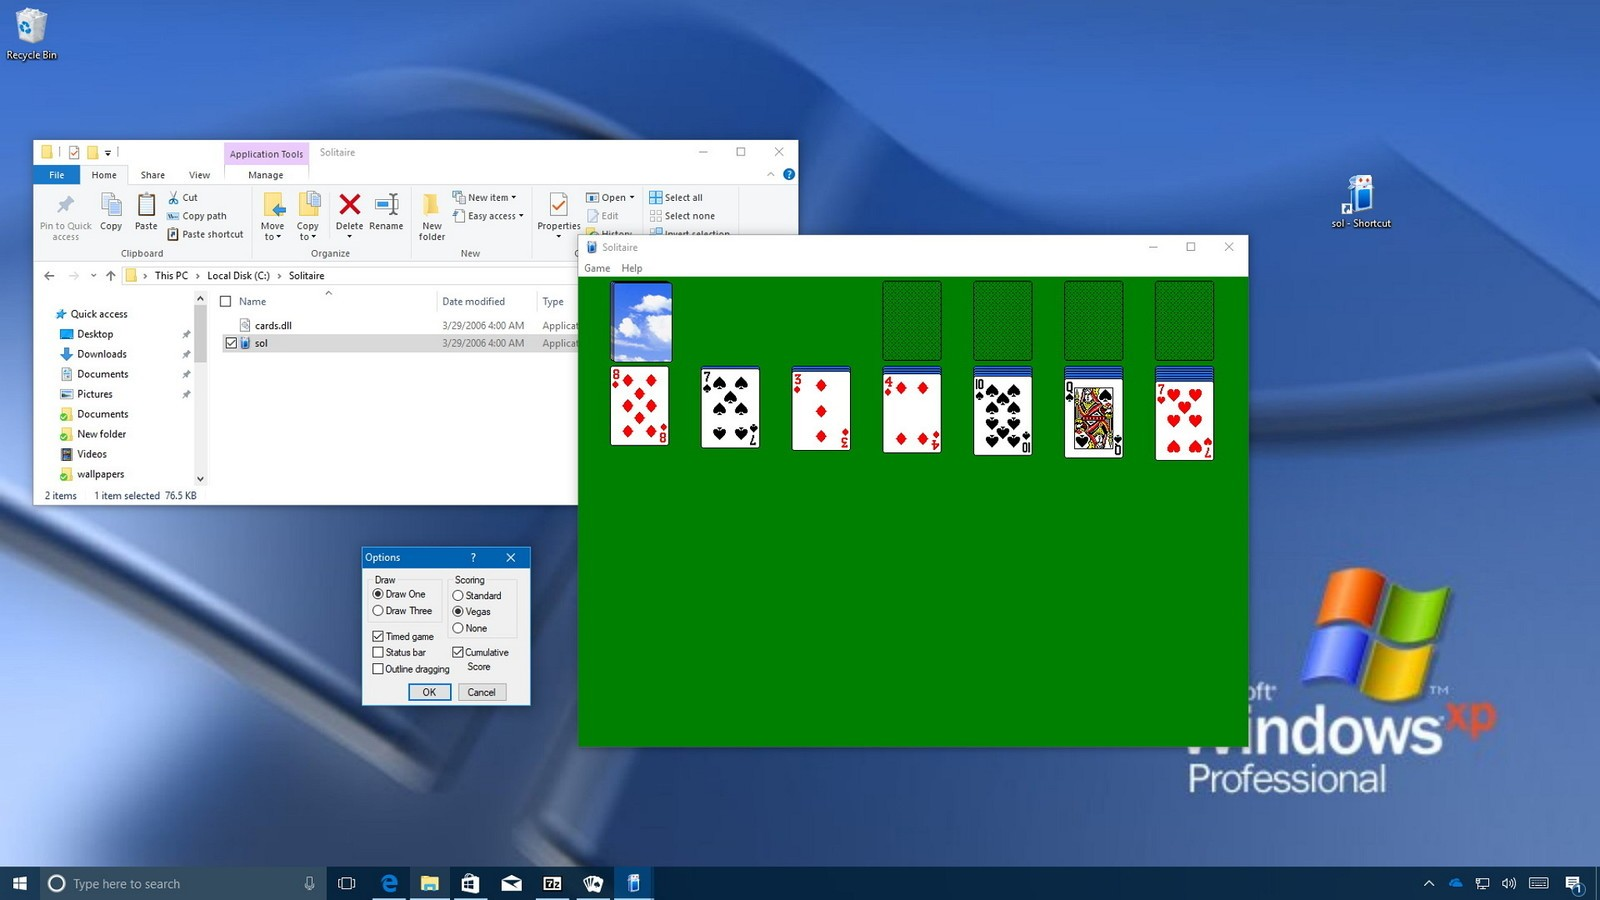
\includegraphics[scale=0.2]{images/windows.jpg} 
     	%\vspace*{-0.5em}
		%\caption{Floating gate transistor cell}
	\end{figure}
	
	\end{center}	
	
		
	\end{frame}	
	
	\begin{frame}
	
	What you will always use after this course:
	
	\begin{center}
		
	\begin{figure}
		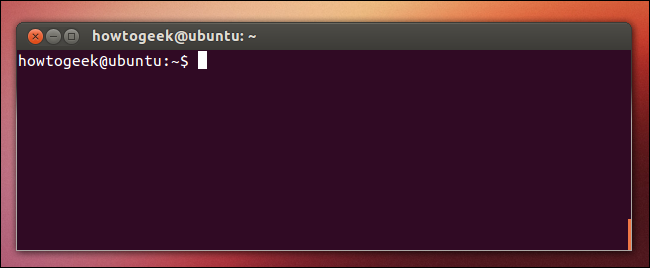
\includegraphics[scale=0.7]{images/terminal.png} 
     	%\vspace*{-0.5em}
		%\caption{Floating gate transistor cell}
	\end{figure}
	
	\end{center}	
		
	\end{frame}	
	
	\begin{frame}

	The Shell:
	\vspace*{1em}
	
	\begin{itemize}
	\item{Shell is an application that reads command lines
from the keyboard and passes them to the Linux operating
system to be executed}
	\item{When you login to a remote Linux system, using a tool like
ssh, you will automatically be connected to a shell}
	\item{Your computing session is kept separate from other user’s
computing sessions, because they are “enclosed” in a
“shell”}
	\item{On your desktop, laptop, or tablet, you may have to find and
execute a terminal emulator application to bring up a shell in
a window}	
	\end{itemize}
		
	\end{frame}	
	
	\begin{frame}
	
	\begin{center}
		
	\begin{figure}
		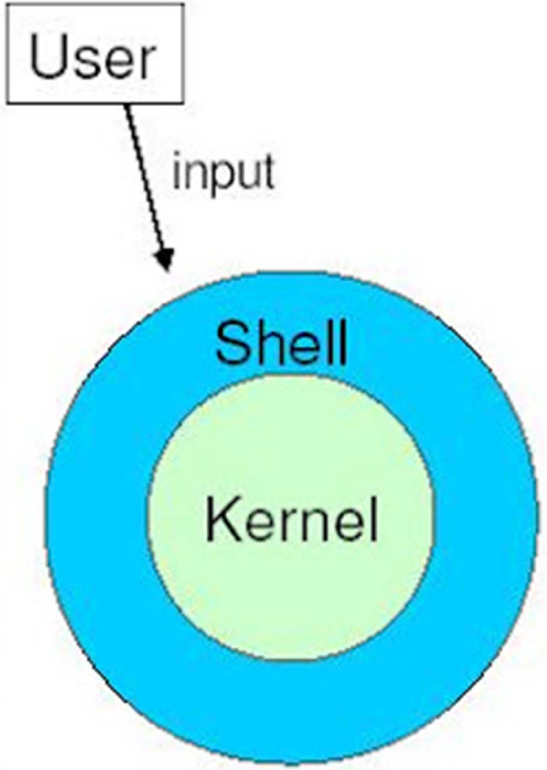
\includegraphics[scale=0.4]{images/shell.png} 
     	%\vspace*{-0.5em}
		%\caption{Floating gate transistor cell}
	\end{figure}
	
	\end{center}		
	
	\begin{exampleblock}{Definition}
	The \textit{Shell} is basically a bridge between kernel and the user. Using \textit{command lines} users can type commands which are conveyed to the kernel and will be executed.	
	\end{exampleblock}	
		
	
	\end{frame}	
	
	\section{The command line}	
	
	\begin{frame}
	
	A basic way of interacting with a Linux system:
	\vspace*{1em}
	\begin{itemize}
	\item{Execute commands}
	\item{Create files and directories}
	\item{Edit file content}
	\item{Access the web}
	\item{Copy files to and from other hosts}
	\item{Run parallel jobs on distant servers}
	\item{etc ...}
	\item{... basically: do things you cannot do as easily with a Graphical User Interface (GUI)}
	\end{itemize}
	
	
	\end{frame}	
	
	\begin{frame}
	
	Why learning the command line?
	\vspace*{1em}
	
	\begin{itemize}
	\item{Linux was designed for the command line}
	\item{You can create new Linux commands using the command
line, without programming}
	\item{Many systems provide only the command line, or poorly
support a GUI interface
	\begin{itemize}
	\item{HPC systems}
	\item{Spark/Hadoop for Big Data}
	\item{etc...}
	\end{itemize}
	}
	\item{Many things can be accomplished only through the
command line
	\begin{itemize}
	\item{Much systems administration \& troubleshooting}
	\end{itemize}
	}

	\pause
	
	\item{Or you just want to look "cool"
	
		\begin{figure}
		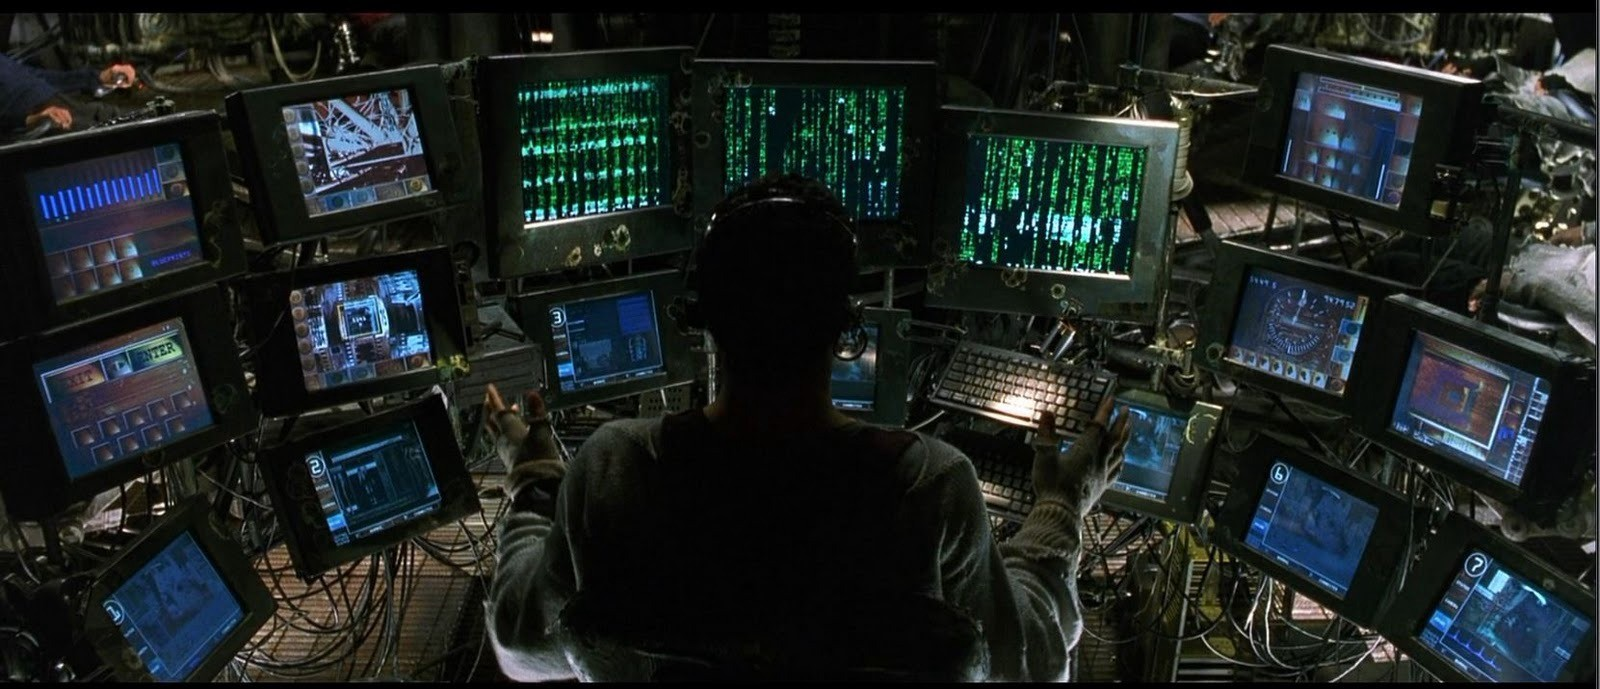
\includegraphics[scale=0.08]{images/cool.jpeg} 
     	%\vspace*{-0.5em}
		%\caption{Floating gate transistor cell}
	\end{figure}
	
	
	}		
	
	
	\end{itemize}
		
	\end{frame}	
	
	\subsection{Accessing a Shell}
	
	\begin{frame}

	To access a Shell you need to use a Terminal Emulator:
	\vspace*{1em}
	\begin{itemize}
	\item{On Linux and Mac OS X: 
		\begin{itemize}
		\item{Just start a terminal (Xterm, Eterm, etc)}
		\item{Use ssh command (if you want to connect to another machine's Shell)}
		\end{itemize}
	}
	\item{On Windows:
		\begin{itemize}
		\item{You can use Cygwin to launch Linux commands on your system}
		\item{Use putty (or mobaxterm) to connect to another machine's Shell}
		\end{itemize}
	}	
	\end{itemize}		
	
	\end{frame}	

	\section{The Shell prompt}

	\begin{frame}
	
	The “user@machine:$\sim$\$“ is the shell prompt
	\vspace*{1em}		
	\begin{itemize}
	\item{This means the shell is waiting for you to type something}
	\item{Format can vary, usually ends with “\$” , “\%” or “\#”
		\begin{itemize}
			\item{If \$ or \%, you have a normal shell
				\begin{itemize}
				\item{This shell has your privileges (rights)}
				\end{itemize}
			}
			\pause			
			{\color{red}
			\item{If \#, you have a so‐called “root shell”
			
			\begin{itemize}
				\item{\color{red} This shell has administrator privileges}	
				\item{\color{red} You can do a great deal of irreversible damage
				
				\begin{figure}
					
\includegraphics[scale=0.4]{images/caution.png} 
     				%\vspace*{-0.5em}
					%\caption{Floating gate transistor cell}
				\end{figure}
				}
			\end{itemize}
			}
			}
		\end{itemize}
	}
	\end{itemize}
	

	\end{frame}		
	
	\section{Typing into the Shell}	
	
	\begin{frame}
	
	Basic input line editing commands:
	\vspace*{1em}
	\begin{itemize}
	\item{Backspace erases previous character}
	\item{Left and right arrow move insertion point on the line}
	\item{Control‐c interrupts whatever command you started and returns}
	\item{you to the shell prompt (usually)}
	\item{Control‐u erases the line from the beginning to the cursor}
	\item{Control‐k erases the line from the cursor to the end}
	\item{Enter executes the line you typed}
	\item{Up and down arrow will access your command history}
	\item{Type “exit” and press Enter without the quotes to exit the shell}
	\item{Click the red "close" icon at the top of the Terminal window to close
	it (on a Mac)}
	\end{itemize}
		
	\end{frame}	
	
	\begin{frame}
	
	Later, as a practical exercise, try these commands and see what happen:
	\vspace*{1em}
	
	\blue{$\sim$\$date}
	
	\blue{$\sim$\$ id}
	
	\blue{$\sim$\$ ps}
	
	\blue{$\sim$\$ df ‐kh}
	
	\blue{$\sim$\$ who}
	
	\blue{$\sim$\$ top} \# type Control‐c or q to exit
	
	\blue{$\sim$\$ history}
		
	\end{frame}		
	
	\section{Navigating the File System}	

	\subsection{Recall}
		
	\begin{frame}
	
	Recall:
	\vspace*{1em}	
	
	\begin{itemize}
	\item{Files are stored in a directory}
	\item{Directories may contain other directories as well as files}
	\item{A hierarchy of directories is called a directory tree}
	\item{A directory tree (a connected graph with no cycles) has a single, topmost root directory}
	\item{A directory tree, rooted at the system root directory “/”, is called a file system}
	\end{itemize}
		
	\end{frame}

	\subsection{Example of a Linux File System}
	
	\begin{frame}
	
	\begin{figure}
		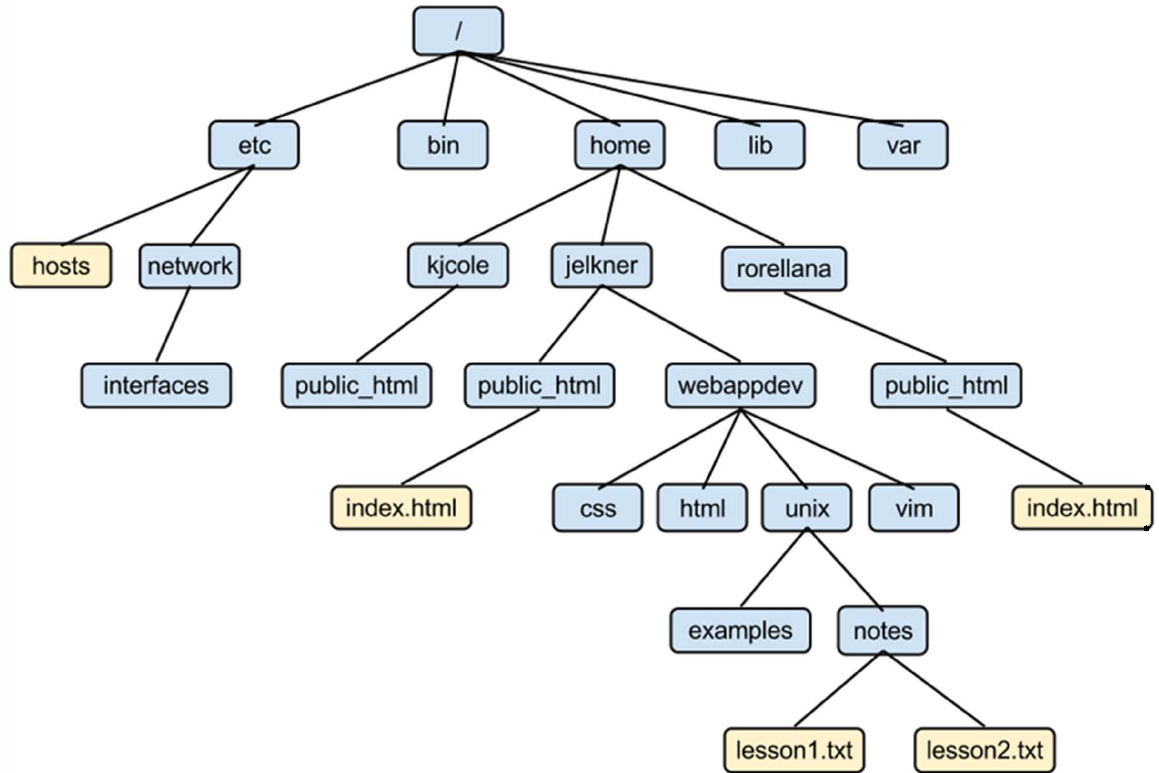
\includegraphics[scale=0.6]{images/fs_example.png} 
     	%\vspace*{-0.5em}
		%\caption{Floating gate transistor cell}
	\end{figure}
	
	\end{frame}
		
	\begin{frame}

	\begin{itemize}
	\item{A file is accessed using its path name}
	\item{Absolute path name
		\begin{itemize}
		\item{/dir1/dir2/.../dirN/filename}
		\item{/usr/X11R6/bin}
		\end{itemize}
	}
	\item{Relative path name
		\begin{itemize}
		\item{current‐working‐directory/filename}
		\end{itemize}
	}
	\item{Every shell maintains a notion of a current working directory
		\begin{itemize}
		\item{Initialized at login to your home directory}
		\item{Changed via cd command}
		\end{itemize}
	}
	\item{Two special directories:
	\begin{itemize}
		\item{. refers to the current directory}
		\item{.. refers to the current directory’s parent directory}
	\end{itemize} 
	}	
	\item{Many ways to get “home”
	\begin{itemize}
		\item{ $\sim$ refers to your home directory}
		\item{ \$HOME is a synonym for $\sim$ }
		\item{ $\sim$username refers to a user’s home directory}
	\end{itemize}
	}	
	\end{itemize}
	
	\end{frame}
	
	\subsection{Basic commands}	
	
	\begin{frame}
	
	Some fundamental commands:
	\vspace*{1em}
	
	\blue{$\sim$\$ file file} \# what kind of file is file?
	
	\blue{$\sim$\$ cat file} \# display contents of text file
	
	\blue{$\sim$\$ less file} \# paginate text file
	
	\blue{$\sim$\$ man command} \# get info about command
	
	\vspace*{1em}	
	
	\begin{block}{Exercise for later}
	Figure out how to make the date command display the date in Coordinated Universal Time (UTC)
	\end{block} 
		
	\end{frame}
	
	\subsection{Navigating the File System}	
	
	\begin{frame}
	
	Some fundamental commands:
	\vspace*{1em}

	\blue{$\sim$\$ pwd} \# print working directory
	
	\blue{$\sim$\$ cd dir} \# make dir the current working directory

	\blue{$\sim$\$ cd} \# cd to your home dir

	\blue{$\sim$\$ cd ~cja} \# cd to cja’s home dir
	
	\blue{$\sim$\$ mkdir dir} \# create directory dir
	
	\blue{$\sim$\$ rmdir dir} \# remove (empty) directory dir

	\blue{$\sim$\$ rm ‐fR dir} \# remove directory dir (empty or not)

	\blue{$\sim$\$ tree} \# display dir tree
		
	\end{frame}	
	
	\begin{frame}
	
	Later, as a practical exercise, try these commands and see what happen:
	\vspace*{1em}
	
	\blue{$\sim$\$ cd} \# make your home directory the current working directory
	
	\blue{$\sim$\$ pwd} \# print working directory
	
	\blue{$\sim$\$ mkdir foo} \# create directory foo
	
	\blue{$\sim$\$ cd foo} \# cd to the foo directory
	
	\blue{$\sim$\$ mkdir bar} \# create directory bar

	\blue{$\sim$\$ cd ..} \# go up one level in the directory tree
	
	\blue{$\sim$\$ tree foo} \# display foo’s directory tree.

	\end{frame}	

	\subsection{Listing info on files}
	
	\begin{frame}
	
	The \textit{ls} command (list information about files)
	\vspace*{1em}
	
	\blue{$\sim$\$ ls} \# list contents of cur dir
	
	\blue{$\sim$\$ ls dir} \# list contents of dir
	
	\blue{$\sim$\$ ls ‐l} \# list details of files in current dir 
	
	\blue{$\sim$\$ ls ‐t} \# list newest files first
	
	\blue{$\sim$\$ ls ‐R dir} \# list all files in tree dir
	
	\blue{$\sim$\$ ls ‐lt dir} \# options can be combined
	
	\blue{$\sim$\$ ls ‐hl dir} \# list all files in human readable
format
	
	\end{frame}
		
	\subsection{Working with files}		
		
	\begin{frame}
	
	These commands manipulate files:
	\vspace*{1em}
	
	\blue{$\sim$\$ mv big large} \# rename file big to large
	
	\blue{$\sim$\$ cp big large} \# copy file big to large
	
	\blue{$\sim$\$ cp ‐r dir1 dir2} \# copy dir tree dir1 to dir2

	\blue{$\sim$\$ cp f1 f2 dir} \# copy file1 and file2 to directory dir

	\blue{$\sim$\$ mkdir dir} \# create empty directory dir

	\pause
	{\color{red}
	$\sim$\$ rmdir dir \# remove empty directory dir

	$\sim$\$ rm file \# remove file file

	$\sim$\$ rm ‐r dir \# remove directory tree dir
	}
	\begin{center}
	\begin{figure}
		
\includegraphics[scale=0.2]{images/caution.png} 
     	%\vspace*{-0.5em}
		%\caption{Floating gate transistor cell}
	\end{figure}
	\end{center}
	
	\end{frame}		
		
	\begin{frame}
	
	Later, as a practical exercise, let's do this:
	\vspace*{1em}
	
	Create a directory named tutorial in your home
	directory. In that directory, create a directory named
	sample and a directory named test . Create a file
	named msg in directory test that contains a copy of the
	file /etc/os‐release.

	\vspace*{1em}

	\begin{block}{Extra credit}
	Make the last‐modified time of your copy
	identical to that of /etc/os‐release. Hint: look at the
	options of the copy command
	\end{block}	
	
	\end{frame}		
		
	\section{Permissions}		
		
	\subsection{Recall}
		
	\begin{frame}

	Recall:
	\vspace*{1em}
	
	\begin{itemize}
	\item{We have three permission types:
	\vspace*{0.5em}
	\begin{itemize}
		\item{Files: Read, Write and Execute}
		\item{Equivalent for directories: List, Modify and Search}
	\end{itemize}}
	\vspace*{1em}
	\item{We have three user classes:
	\vspace*{0.5em}
	\begin{itemize}
	\item{User (File Owner), Group, All (Other)}
	\item{Type: man chmod (for more help)}
	\end{itemize}
	}
	\end{itemize}	
	\end{frame}		
		
	\subsection{Examples}		
		
	\begin{frame}
	
	\begin{center}
	\begin{figure}
		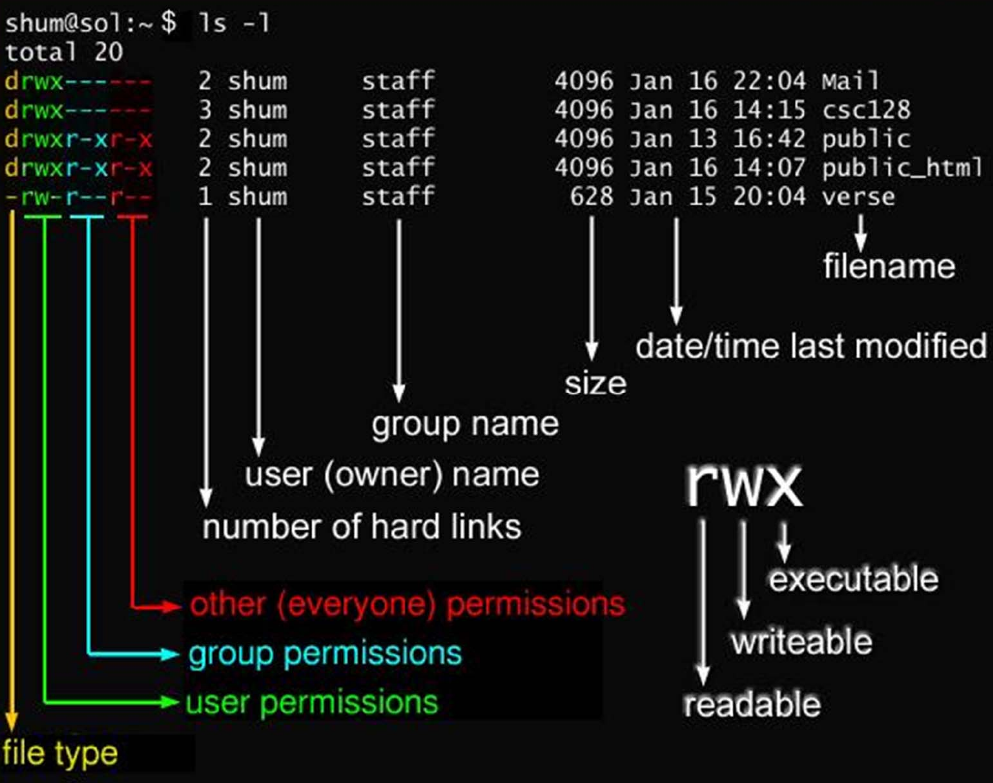
\includegraphics[scale=0.6]{images/permission_example.png} 
     	%\vspace*{-0.5em}
		%\caption{Floating gate transistor cell}
	\end{figure}
	\end{center}	
	
	
	\end{frame}			
	
	\begin{frame}
	
	Other examples:
	\vspace*{1em}	
	
	‐rw‐‐‐‐‐‐‐ cja lsait 40 Oct 1 12:03 foo.bz2
	\vspace*{0.2em}
	
	file read and write rights for the owner, no access for
anyone else 
	\vspace*{1em}
	
	‐rw‐r‐‐‐‐‐ cja lsait 40 Oct 1 12:03 foo.bz2
	\vspace*{0.2em}
	
	file read and write rights for the owner, read for
	members of the lsait group and no access for others
	(we typed: chmod u=rw,g=r,o= foo.bz2)
	\vspace*{1em}

	drwxr‐x‐‐x cja lsait 4096 Oct 1 12:15 bar
	\vspace*{0.2em}
	
	list, modify, and search for the owner, list and search
	for group, and execute only for others
	
	\end{frame}
	
%	\begin{frame}
%	
%	Later, as a practical exercise, try these commands and see what happen:
%	\vspace*{1em}
%	
%	\~\ \$ cd \# make your home directory the current working directory
%	
%	\~\ \$ pwd \# print working directory to verify you are in your home directory
%	
%	\~\ \$ mkdir training \# create directory training
%	
%	\~\ \$ cd training \# cd to the training directory
%
%	\~\ \$ cp ‐rf /data/examples/IntroLinux/. . \# copies sample files to training directory
%		
%	\end{frame}	

	\section{Compression, archiving and wildcards}
	
	\subsection{Compressing and archiving}
	
	\begin{frame}
	
	These commands compress and archive files:
	\vspace*{1em}
	
	\blue{$\sim$\$ gzip foo} \# compress foo to foo.gz

	\blue{$\sim$\$ gunzip foo} \# uncompress foo.gz to foo
	
	\blue{$\sim$\$ bzip2 foo} \# better compress foo to foo.bz2

	\blue{$\sim$\$ bunzip2 foo} \# uncompress foo.bz2 to foo
	
	\blue{$\sim$\$ tar ‐cf foo.tar bar} \# archive subtree bar in file foo.tar
	
	\blue{$\sim$\$ tar ‐xf foo.tar} \# restore archive from file foo.tar

	\blue{$\sim$\$ tar ‐tf foo.tar} \# list files in archive file foo.tar

	\blue{$\sim$\$ tar ‐zcf foo.tgz bar} \# archive and compress
	
	\blue{$\sim$\$ tar ‐jcf foo.tjz bar} \# archive and compress better
	
	\vspace*{1em}
	\begin{block}{Exercise for later}
	Archive and compress files in a directory to a file
named example.tgz
	\end{block}	
	
	\end{frame}
		
	\subsection{Wildcards}		
		
	\begin{frame}
	
	The Shell accepts wildcarded arguments (also called "shell globbing")
	\vspace*{1em}	
	
	Wildcards:
	\vspace*{0.5em}
	
	\begin{itemize}
	\item{? Matches a single character}
	\item{* Matches zero or more characters}
	\item{[chars] Matches any of the chars}
	\item{[c1‐c2] Matches chars ‘c1’ through ‘c2’}
	\item{[$\sim$chars] Matches any but the chars}
	\end{itemize}
	\vspace*{1em}
	
	\blue{$\sim$\$ ls foo.?} \# match files named foo.x, where x is any character

	\blue{$\sim$\$ echo \*.[cs]} \# echo files that end in .c or .s
	
	\blue{$\sim$\$ mv [o‐z]* save} \# move files starting with o through z to directory save

	\blue{$\sim$\$ echo [$\sim$A‐Z]?} \# ???
		
	\end{frame}		
			
	\section{Shell redirection \& Pipeline}
	\subsection{Shell redirection}	
	
	\begin{frame}
	
	A Linux command can have its inputs and outputs redirected:
	\vspace*{1em}
	
	\blue{$\sim$\$ ls >myfiles} \# put list of files in current directory into file myfiles
	
	\blue{$\sim$\$ ls >>filelist} \# add list of files in current directory to end of file filelist
	
	\blue{$\sim$\$ sort <grocery.list} \# sort lines from file grocery.list

	\blue{$\sim$\$ sort <<EOF} 
	
\blue{whiskey}

\blue{bravo}

\blue{tango}

\blue{EOF} \# sort lines entered at keyboard

	\blue{$\sim$\$ wc ‐l </etc/os‐release >$\sim$/mycounts} \# count number of lines from file /etc/os‐release and put result in file mycounts in my home directory
	
		
	\end{frame}
	
	\subsection{Useful commands used with redirection and pipelines}	
	
	\begin{frame}
	
	More useful Linux tool commands used for redirection and pipelines:
	\vspace*{1em}

	\blue{$\sim$\$ grep string} \# show lines of input containing string
	
	\blue{$\sim$\$ tail} \# show last few lines of input
	
	\blue{$\sim$\$ head} \# show first few lines of input
	
	\blue{$\sim$\$ sort} \# sort the input

	\blue{$\sim$\$ du ‐sh} \# report the size of the current directory
	
	\blue{$\sim$\$ du ‐sh dir} \# report the size of directory dir

	\blue{$\sim$\$ who} \# gives a list of the users currently logged in

	\blue{$\sim$\$ cut ‐cxx ‐yy} \# keep the output from a command starting at the xx character in the line and ending
at the yy character
		
	\end{frame}	
	
	\subsection{Pipelines}	
	
	\begin{frame}
	
	A Linux command can have its output connected to the input of another Linux command:
	\vspace*{1em}
	
	\blue{$\sim$\$ ls | wc –l} \# count files in current directory

	\blue{$\sim$\$ last | grep reboot} \# when did we reboot?
	
	\vspace*{1em}
	\begin{block}{Exercises for later}
	\begin{itemize}
	\item{How many users are currently logged in?}
	\item{How many unique user IDs are currently logged in?}
	\end{itemize}
	\end{block}
	
	\end{frame}	
			
	\section{Editing text files}
		
	\begin{frame}
	
	
	Simple editor:
	\vspace*{1em}
	
	\begin{itemize}
	\item{nano
	\begin{itemize}
	\item{Simple to learn if you want to get started quickly}
	\item{No mouse support. Arrow keys for navigation}
	\end{itemize}
	}
	\end{itemize}
	\vspace*{0.5em}
	
	Supported editors:
	\vspace*{1em}
	
	\begin{itemize}
	\item{vi, vim or emacs
		\begin{itemize}
			\item{Powerful but more complex}
			\item{If you have time and inclination to become proficient}
		\end{itemize}
	}
	\end{itemize}
		
	\end{frame}		
	
	\begin{frame}

	\begin{alertblock}{Warning}
	Watch out for source code or data files written on Windows systems
	\end{alertblock}
		
	\vspace*{1em}
	Use these tools to analyze and convert source files to Linux format:
	\vspace*{1em}
	
	\begin{itemize}
		\item{file}
		\item{dos2unix}
		\item{unix2dos}
	\end{itemize}
	
	\end{frame}
	
	\section{File transfers}
	
	\begin{frame}
	
	Eventually, you will need to move/copy files to and from your computer and a server/workstation/cluster. You can do this using the secure copy command (scp) in a terminal window.
	\vspace*{1em}	
	
	To transfer files (foobar.txt) FROM your local host TO a remote host use:
	\vspace*{0.5em}

	\blue{$\sim$\$ scp foobar.txt $username@remotehost.edu$:/some/remote/directory} 
	\vspace*{0.5em}	
	
	To transfer files (foobar.txt) FROM a remote host TO your local host use:
	\vspace*{0.5em}	
	
	\blue{$\sim$\$ scp $username@remotehost.edu$:foobar.txt /some/local/directory}
	\vspace*{0.5em}	
	
	To copy a directory, repeat as above adding the ‐r flag. ($\sim$\$ scp ‐r ... )
	\vspace*{0.5em}

	Graphical, drag‐and‐drop scp programs are available for Windows and Mac platforms.
	(WinSCP – Windows, Cyberduck – Mac)
	
	\end{frame}		
			
	\begin{frame}
	
	Modern operating systems are usually multitasking, meaning that they create the illusion of doing more than one thing at once by rapidly switching from one executing program to another. The Linux kernel manages this through the use of processes. Processes are how Linux organizes the different programs waiting for their turn at the CPU.
	\vspace*{1em}
	\begin{itemize}
	\item{On Linux, every program runs in a process}
	\item{You can examine these processes}
\end{itemize}
\vspace*{1em}

	Commands on processes:
	\vspace*{1em}
	
	\blue{$\sim$\$ man ps}
	
	\blue{$\sim$\$ ps}
	
	\blue{$\sim$\$ ps ax}

	\blue{$\sim$\$ top}

	\pause
	
	{\color{red}
	$\sim$\$ man kill
	
	$\sim$\$ kill PID	

	\begin{center}
	\begin{figure}
		
\includegraphics[scale=0.08]{images/caution.png} 
     	%\vspace*{-0.5em}
		%\caption{Floating gate transistor cell}
	\end{figure}
	\end{center}

	}	
		
	\end{frame}			
	
	\section{Additional commands}	
	
	\begin{frame}
	
	Additional interesting commands:
	\vspace*{1em}
	
\blue{$\sim$\$ quota ‐Q ‐s \$USER} \# show disk quota for \$USER

\blue{$\sim$\$ grep “sometext” somefile} \# find \& print sometext if found in somefile

\blue{$\sim$\$ history} \# displays last n commands entered

\blue{$\sim$\$ clear} \# clears the screen

\blue{$\sim$\$ diff ‐w file1 file2} \# compare file1 with file2 ignoring all white space

\blue{$\sim$\$ which command} \# prints the full path to command

\blue{$\sim$\$ acommand | tee filename} \# takes the results from acommand and prints them to the screen and to the file filename (Use tee –a to append to filename)

\blue{$\sim$\$ source filename} \# reads and executes the commands contained in filename


\end{frame}

\section{Environment Variables}
\subsection{Principle}
\begin{frame}

An environment variable is a named object that contains data used by
one or more applications. In simple terms, it is a variable with a name
and a value.
\vspace*{0.5em}

The convention in Linux is for the environment variable to be all
uppercase letters.
\vspace*{0.5em}

To use an environment variable, prefix the variable name with \$.
You can see the value of an environment variable by typing:
\vspace*{1em}

\blue{$\sim$\$ echo \$VARIABLENAME}
\vspace*{1em}

You can see all the environment variables defined for your session by typing:
\vspace*{0.5em} 

\blue{$\sim$\$ env}
\vspace*{0.5em} 

You can set an environment variable by typing:

\blue{$\sim$\$ export VARIABLENAME = value}


\end{frame}

\subsection{Common environment variables}			
\begin{frame}

Common environment variables:
\vspace*{1em}

USER \# \$USER ‐‐> user login name

PATH \# \$PATH ‐‐> a list of directories to look into for programs and files

HISTSIZE \# \$HISTSIZE ‐‐> number of commands to keep in history

HOSTNAME \# \$HOSTNAME ‐‐> fully enumerated host name

HOME \# \$HOME ‐‐> home directory of the user

TERM \# \$TERM ‐‐> terminal type

SHELL \# \$SHELL ‐‐> shell type you are using

\end{frame}			
			
\section{More commands and tips...}
			
\begin{frame}

You can find more commands and tips in the "Linux Command Line" book: 
\vspace*{1em}

http://www.linuxzasve.com/preuzimanje/TLCL-09.12.pdf

\end{frame}
			
			
\end{document}
